
\subsection{LCA}

\begin{frame}
  \frametitle{Mandatory LCA slide (again)}

  \centering
  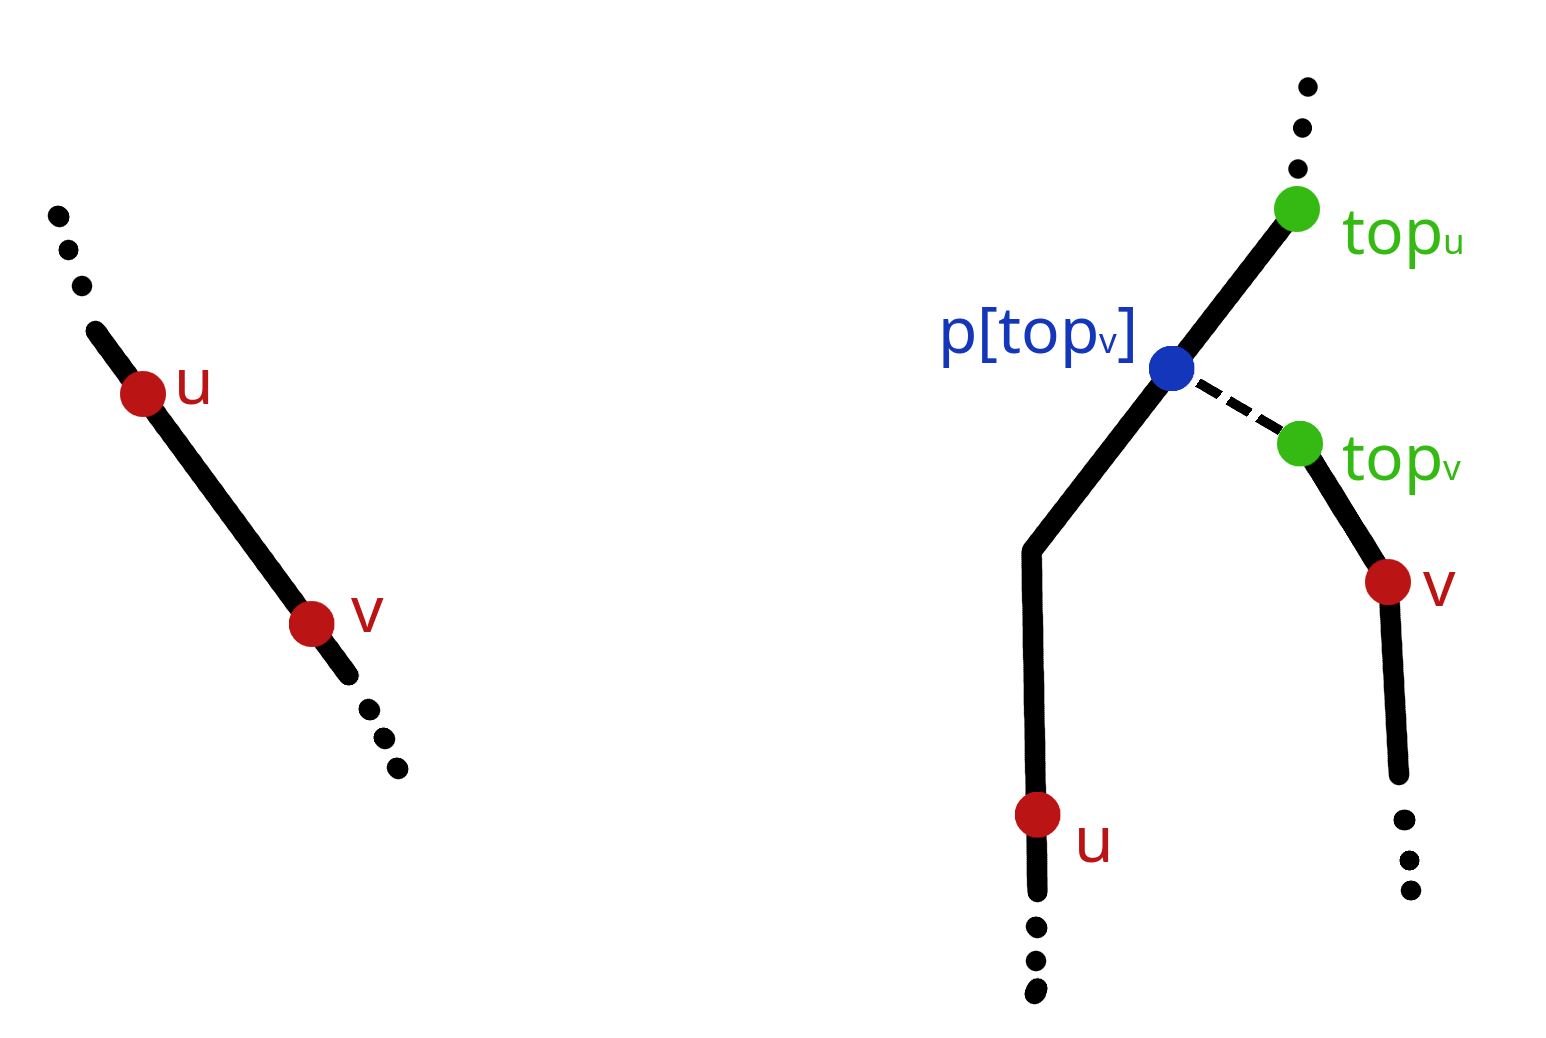
\includegraphics[height=0.85\textheight,keepaspectratio]{fotos/lca.png}
\end{frame}

\begin{frame}[fragile]
  \frametitle{Mandatory LCA slide (again)}
  \begin{lstlisting}
int lca(int u, int v) {
    int tu = htop[u], tv = htop[v];
    if (tu == tv) {
        if (dep[u] > dep[v]) swap(u, v);
        return u;
    } else {
        if (dep[tu] < dep[tv]) swap(u, v), swap(tu, tv);
        return lca(p[tu], v)
    }
}
  \end{lstlisting}
\end{frame}